\documentclass{article}
\setlength{\oddsidemargin}{0.25 in}
\setlength{\evensidemargin}{-0.25 in}
\setlength{\topmargin}{-0.6 in}
\setlength{\textwidth}{6.5 in}
\setlength{\textheight}{8.5 in}
\setlength{\headsep}{0.75 in}
\setlength{\parindent}{0 in}
\setlength{\parskip}{0.1 in}

\usepackage{amsmath,amsfonts,graphicx}
\usepackage{tikz}
\usepackage{epsfig}
\usepackage{filecontents}
\usepackage{pgfplots, pgfplotstable}
\usepackage{mathtools}
\usepackage{breqn}
%\usepackage{fourier}
\usepgfplotslibrary{statistics}
\newcounter{lecnum}
\renewcommand{\thepage}{\thelecnum-\arabic{page}}
\renewcommand{\thesection}{\thelecnum.\arabic{section}}
\renewcommand{\theequation}{\thelecnum.\arabic{equation}}
\renewcommand{\thefigure}{\thelecnum.\arabic{figure}}
\renewcommand{\thetable}{\thelecnum.\arabic{table}}

\newcommand{\lecture}[4]{
  \pagestyle{myheadings}
  \thispagestyle{plain}
  \setcounter{lecnum}{#1}
  \setcounter{page}{1}
  \noindent
  \begin{center}
    \framebox{
      \vbox{\vspace{2mm}
        \hbox to 6.28in { {\bf Analysis of Uncertainties
	    \hfill Fall 2014} }
        \vspace{4mm}
        \hbox to 6.28in { {\Large \hfill Lecture #1: #2  \hfill} }
        \vspace{2mm}
        \hbox to 6.28in { {\it Lecturer: #3 \hfill Notes by: #4} }
        \vspace{2mm}}
    }
  \end{center}
  \markboth{Lecture #1: #2}{Lecture #1: #2}
  \vspace*{4mm}
}

\renewcommand{\cite}[1]{[#1]}
\def\beginrefs{\begin{list}%
    {[\arabic{equation}]}{\usecounter{equation}
      \setlength{\leftmargin}{2.0truecm}\setlength{\labelsep}{0.4truecm}%
      \setlength{\labelwidth}{1.6truecm}}}
\def\endrefs{\end{list}}
\def\bibentry#1{\item[\hbox{[#1]}]}

\newtheorem{theorem}{Theorem}[lecnum]
\newtheorem{lemma}[theorem]{Lemma}
\newtheorem{proposition}[theorem]{Proposition}
\newtheorem{claim}[theorem]{Claim}
\newtheorem{corollary}[theorem]{Corollary}
\newtheorem{definition}[theorem]{Definition}
\newenvironment{proof}{{\bf Proof:}}{\hfill\rule{2mm}{2mm}}

\newcommand\E{\mathbb{E}}


\begin{document}
\lecture{1}{20 October 2014}{Prof. Kate Scholberg}{Douglas Davis}
\section{Introduction}
Think about the value for Newton's gravitational constant $G$; the current accepted value in literature is something around (call it $G_{\text{m1}}$, this doesn't have to be correct we're just making a point).
$$ G_{\text{m1}} = (6.674215\pm0.000092) \times 10^{11} \text{ m}^3\text{ kg}^{-1}\text{ s}^{-2}. $$
Now imagine we perform some experiments where we measure $G$. Imagine we measure a a new value, call it $G_{\text{m2}}$,
$$ G_{\text{m2}} = (6.674400\pm0.000010) \times 10^{11} \text{ m}^3\text{ kg}^{-1}\text{ s}^{-2}. $$
And we measure another value, $G_{\text{m3}}$,
$$ G_{\text{m3}} = (6.6741\pm0.0221) \times 10^{11} \text{ m}^3\text{ kg}^{-1}\text{ s}^{-2}. $$
If we look closely at the values and the uncertainties, we see that the value $G_{\text{m2}}$ is in disagreement with $G_{\text{m1}}$, because the values do not lie within the other value's uncertainty. This means some further investigation is needed! If we look at $G_{\text{m3}}$, we see that it is in agreement with both $G_{\text{m1}}$ and $G_{\text{m1}}$, but the uncertainty is so large that this measurement really did nothing for the advancement of science. This can be seen graphically in Figure~\ref{fig:G}.
\begin{figure}[h!]
  \centerline{
    \begin{tikzpicture}
      \draw [->] (0,0) -- (4,0);
      \draw [->] (0,0) -- (0,3);
      \node at (2,-.85) {Measurements};
      \node at (-.5,1.5) {$G$};
      \node at (1,-.35) {1};
      \node at (2,-.35) {2};
      \node at (3,-.35) {3};
      \draw [|-|,dashed,blue] (1,.9) -- (1,1.9);
      \draw [|-|,dashed,blue] (2,2.2)-- (2,2.6);
      \draw [<->,dashed,blue] (3,.1) -- (3,2.9);
      \draw [fill=red] (1,1.4) circle (2pt);
      \draw [fill=red] (2,2.4) circle (2pt);
      \draw [fill=red] (3,1.0) circle (2pt);
    \end{tikzpicture}
  }
  \caption{Three measurements for $G$, the values are red bullets, and the uncertainties are shown with blue dashed error bars}
  \label{fig:G}
\end{figure}
The point of this example is to show that uncertainties seriously matter. When interpreting results and planning new experiments, a scientist must always be thinking about uncertainties. Why build an experiment if the expected uncertainty in the measurement will yield nothing better than what is already known? Or, what does this new measurement mean that is it so much more constrained than the previous measurement? Is this method so great we should expand it elsewhere, and why is it so much better?

\section{Important Definitions}
Our first two important definitions are \emph{statistical} and \emph{systematic uncertainties}. A \emph{statistical uncertainty} is a random uncertainty that arises simply from random fluctuations in the data. As the sample size of the data approaches infinity ($N \rightarrow \infty$), the statistical uncertainty approaches 0. A \emph{systematic uncertainty} comes from a lack of knowledge about the experimental apparatus/measurement. An example would be the possibly of an inexact measurement from an imperfect ruler. Systematic uncertainties can also have some randomness, if an apparatus is affected by temperature change, the random fluctuations of temperature in the room cause systematic uncertainties because of the effect on the apparatus. To quote the systematic and statistical uncertainties, results are often written in the form:
\begin{align}
  x \pm \Delta x\,(\text{sys.}) \pm \Delta x\,(\text{stat.}),
\end{align}
with the two values separate. As the amount of data increases, the statistical uncertainty always decreases. The same cannot be said for systematic. In theory, studying systematic uncertainties more thoroughly may lead to a decrease, but it is possible that a better understanding of the systematics may cause an increase in the uncertainty.
\noindent Our next definition is a \emph{sample}. The \emph{sample} is the collection of measurements. If we want to measure some value $x$, then the sample is simply:
$$x_1,\,x_2,\,x_3,\,...\,,\,x_N,$$
where $x_i$ is just the $i$th measurement. An infinite number of measurements would yield the sample's \emph{parent distribution}, which we denote with $P(x)$. Figure~\ref{fig:sample,parent} shows an example of a histogrammed sample with it's parent distribution. As $N\rightarrow\infty$, the shape of the histogram would approach the shape of $P(x)$.

\begin{figure}[h!]
  \centerline{
    \begin{tikzpicture}[scale=.5]
\pgfdeclareplotmark{cross} {
\pgfpathmoveto{\pgfpoint{-0.3\pgfplotmarksize}{\pgfplotmarksize}}
\pgfpathlineto{\pgfpoint{+0.3\pgfplotmarksize}{\pgfplotmarksize}}
\pgfpathlineto{\pgfpoint{+0.3\pgfplotmarksize}{0.3\pgfplotmarksize}}
\pgfpathlineto{\pgfpoint{+1\pgfplotmarksize}{0.3\pgfplotmarksize}}
\pgfpathlineto{\pgfpoint{+1\pgfplotmarksize}{-0.3\pgfplotmarksize}}
\pgfpathlineto{\pgfpoint{+0.3\pgfplotmarksize}{-0.3\pgfplotmarksize}}
\pgfpathlineto{\pgfpoint{+0.3\pgfplotmarksize}{-1.\pgfplotmarksize}}
\pgfpathlineto{\pgfpoint{-0.3\pgfplotmarksize}{-1.\pgfplotmarksize}}
\pgfpathlineto{\pgfpoint{-0.3\pgfplotmarksize}{-0.3\pgfplotmarksize}}
\pgfpathlineto{\pgfpoint{-1.\pgfplotmarksize}{-0.3\pgfplotmarksize}}
\pgfpathlineto{\pgfpoint{-1.\pgfplotmarksize}{0.3\pgfplotmarksize}}
\pgfpathlineto{\pgfpoint{-0.3\pgfplotmarksize}{0.3\pgfplotmarksize}}
\pgfpathclose
\pgfusepathqstroke
}
\pgfdeclareplotmark{cross*} {
\pgfpathmoveto{\pgfpoint{-0.3\pgfplotmarksize}{\pgfplotmarksize}}
\pgfpathlineto{\pgfpoint{+0.3\pgfplotmarksize}{\pgfplotmarksize}}
\pgfpathlineto{\pgfpoint{+0.3\pgfplotmarksize}{0.3\pgfplotmarksize}}
\pgfpathlineto{\pgfpoint{+1\pgfplotmarksize}{0.3\pgfplotmarksize}}
\pgfpathlineto{\pgfpoint{+1\pgfplotmarksize}{-0.3\pgfplotmarksize}}
\pgfpathlineto{\pgfpoint{+0.3\pgfplotmarksize}{-0.3\pgfplotmarksize}}
\pgfpathlineto{\pgfpoint{+0.3\pgfplotmarksize}{-1.\pgfplotmarksize}}
\pgfpathlineto{\pgfpoint{-0.3\pgfplotmarksize}{-1.\pgfplotmarksize}}
\pgfpathlineto{\pgfpoint{-0.3\pgfplotmarksize}{-0.3\pgfplotmarksize}}
\pgfpathlineto{\pgfpoint{-1.\pgfplotmarksize}{-0.3\pgfplotmarksize}}
\pgfpathlineto{\pgfpoint{-1.\pgfplotmarksize}{0.3\pgfplotmarksize}}
\pgfpathlineto{\pgfpoint{-0.3\pgfplotmarksize}{0.3\pgfplotmarksize}}
\pgfpathclose
\pgfusepathqfillstroke
}
\pgfdeclareplotmark{newstar} {
\pgfpathmoveto{\pgfqpoint{0pt}{\pgfplotmarksize}}
\pgfpathlineto{\pgfqpointpolar{44}{0.5\pgfplotmarksize}}
\pgfpathlineto{\pgfqpointpolar{18}{\pgfplotmarksize}}
\pgfpathlineto{\pgfqpointpolar{-20}{0.5\pgfplotmarksize}}
\pgfpathlineto{\pgfqpointpolar{-54}{\pgfplotmarksize}}
\pgfpathlineto{\pgfqpointpolar{-90}{0.5\pgfplotmarksize}}
\pgfpathlineto{\pgfqpointpolar{234}{\pgfplotmarksize}}
\pgfpathlineto{\pgfqpointpolar{198}{0.5\pgfplotmarksize}}
\pgfpathlineto{\pgfqpointpolar{162}{\pgfplotmarksize}}
\pgfpathlineto{\pgfqpointpolar{134}{0.5\pgfplotmarksize}}
\pgfpathclose
\pgfusepathqstroke
}
\pgfdeclareplotmark{newstar*} {
\pgfpathmoveto{\pgfqpoint{0pt}{\pgfplotmarksize}}
\pgfpathlineto{\pgfqpointpolar{44}{0.5\pgfplotmarksize}}
\pgfpathlineto{\pgfqpointpolar{18}{\pgfplotmarksize}}
\pgfpathlineto{\pgfqpointpolar{-20}{0.5\pgfplotmarksize}}
\pgfpathlineto{\pgfqpointpolar{-54}{\pgfplotmarksize}}
\pgfpathlineto{\pgfqpointpolar{-90}{0.5\pgfplotmarksize}}
\pgfpathlineto{\pgfqpointpolar{234}{\pgfplotmarksize}}
\pgfpathlineto{\pgfqpointpolar{198}{0.5\pgfplotmarksize}}
\pgfpathlineto{\pgfqpointpolar{162}{\pgfplotmarksize}}
\pgfpathlineto{\pgfqpointpolar{134}{0.5\pgfplotmarksize}}
\pgfpathclose
\pgfusepathqfillstroke
}
\definecolor{c}{rgb}{1,1,1};
\draw [color=c, fill=c] (0,0) rectangle (20,13.592);
\draw [color=c, fill=c] (2,1.3592) rectangle (18,12.2328);
\definecolor{c}{rgb}{0,0,0};
\draw [c] (2,1.3592) -- (2,12.2328) -- (18,12.2328) -- (18,1.3592) -- (2,1.3592);
\definecolor{c}{rgb}{1,1,1};
\draw [color=c, fill=c] (2,1.3592) rectangle (18,12.2328);
\definecolor{c}{rgb}{0,0,0};
\draw [c] (2,1.3592) -- (2,12.2328) -- (18,12.2328) -- (18,1.3592) -- (2,1.3592);
\definecolor{c}{rgb}{0,0,0.6};
\draw [c] (2,1.3592) -- (3.6,1.3592) -- (3.6,1.48001) -- (5.2,1.48001) -- (5.2,1.60083) -- (6.8,1.60083) -- (6.8,5.10453) -- (8.4,5.10453) -- (8.4,10.4205) -- (10,10.4205) -- (10,9.57478) -- (11.6,9.57478) -- (11.6,3.41309) -- (13.2,3.41309) --
 (13.2,1.96328) -- (14.8,1.96328) -- (14.8,1.48001) -- (16.4,1.48001) -- (16.4,1.3592) -- (18,1.3592);
\definecolor{c}{rgb}{1,0,0};
\draw [c,line width=0.4] (2.08,1.3592) -- (2.24,1.3592) -- (2.4,1.3592) -- (2.56,1.3592) -- (2.72,1.3592) -- (2.88,1.3592) -- (3.04,1.3592) -- (3.2,1.3592) -- (3.36,1.3592) -- (3.52,1.36055) -- (3.68,1.36132) -- (3.84,1.36247) -- (4,1.3642) --
 (4.16,1.36675) -- (4.32,1.37047) -- (4.48,1.37583) -- (4.64,1.38346) -- (4.8,1.39418) -- (4.96,1.40907) -- (5.12,1.42949) -- (5.28,1.45713) -- (5.44,1.49409) -- (5.6,1.54288) -- (5.76,1.60646) -- (5.92,1.68825) -- (6.08,1.79211) -- (6.24,1.92226) --
 (6.4,2.08318) -- (6.56,2.27948) -- (6.72,2.51567) -- (6.88,2.7959) -- (7.04,3.12369) -- (7.2,3.50156) -- (7.36,3.93069) -- (7.52,4.41059) -- (7.68,4.93876) -- (7.84,5.51048) -- (8,6.11862) -- (8.16,6.75364) -- (8.32,7.40367) -- (8.48,8.0548) --
 (8.64,8.69151) -- (8.8,9.29722) -- (8.96,9.85498) -- (9.12,10.3483) -- (9.28,10.7617) -- (9.44,11.0821) -- (9.6,11.2987) -- (9.76,11.4044) -- (9.92,11.3954);
\draw [c,line width=0.4] (9.92,11.3954) -- (10.08,11.272) -- (10.24,11.0386) -- (10.4,10.7029) -- (10.56,10.276) -- (10.72,9.77154) -- (10.88,9.20516) -- (11.04,8.59349) -- (11.2,7.95344) -- (11.36,7.30149) -- (11.52,6.65294) -- (11.68,6.02141) --
 (11.84,5.4184) -- (12,4.85309) -- (12.16,4.33222) -- (12.32,3.86015) -- (12.48,3.43906) -- (12.64,3.06914) -- (12.8,2.74899) -- (12.96,2.4759) -- (13.12,2.24624) -- (13.28,2.05578) -- (13.44,1.89998) -- (13.6,1.77423) -- (13.76,1.6741) --
 (13.92,1.5954) -- (14.08,1.53434) -- (14.24,1.48759) -- (14.4,1.45225) -- (14.56,1.42586) -- (14.72,1.40641) -- (14.88,1.39226) -- (15.04,1.38208) -- (15.2,1.37486) -- (15.36,1.36979) -- (15.52,1.36628) -- (15.68,1.36388) -- (15.84,1.36226) --
 (16,1.36117) -- (16.16,1.36046) -- (16.32,1.3592) -- (16.48,1.3592) -- (16.64,1.3592) -- (16.8,1.3592) -- (16.96,1.3592) -- (17.12,1.3592) -- (17.28,1.3592) -- (17.44,1.3592) -- (17.6,1.3592) -- (17.76,1.3592);
\draw [c,line width=0.4] (17.76,1.3592) -- (17.92,1.3592);
\definecolor{c}{rgb}{0,0,0};
\draw [c] (2,1.3592) -- (18,1.3592);
\draw (10,0.198046) node[scale=1, rotate=0]{$x$};
\draw [c] (2,1.6854) -- (2,1.3592);
\draw [c] (2.32,1.5223) -- (2.32,1.3592);
\draw [c] (2.64,1.5223) -- (2.64,1.3592);
\draw [c] (2.96,1.5223) -- (2.96,1.3592);
\draw [c] (3.28,1.5223) -- (3.28,1.3592);
\draw [c] (3.6,1.6854) -- (3.6,1.3592);
\draw [c] (3.92,1.5223) -- (3.92,1.3592);
\draw [c] (4.24,1.5223) -- (4.24,1.3592);
\draw [c] (4.56,1.5223) -- (4.56,1.3592);
\draw [c] (4.88,1.5223) -- (4.88,1.3592);
\draw [c] (5.2,1.6854) -- (5.2,1.3592);
\draw [c] (5.52,1.5223) -- (5.52,1.3592);
\draw [c] (5.84,1.5223) -- (5.84,1.3592);
\draw [c] (6.16,1.5223) -- (6.16,1.3592);
\draw [c] (6.48,1.5223) -- (6.48,1.3592);
\draw [c] (6.8,1.6854) -- (6.8,1.3592);
\draw [c] (7.12,1.5223) -- (7.12,1.3592);
\draw [c] (7.44,1.5223) -- (7.44,1.3592);
\draw [c] (7.76,1.5223) -- (7.76,1.3592);
\draw [c] (8.08,1.5223) -- (8.08,1.3592);
\draw [c] (8.4,1.6854) -- (8.4,1.3592);
\draw [c] (8.72,1.5223) -- (8.72,1.3592);
\draw [c] (9.04,1.5223) -- (9.04,1.3592);
\draw [c] (9.36,1.5223) -- (9.36,1.3592);
\draw [c] (9.68,1.5223) -- (9.68,1.3592);
\draw [c] (10,1.6854) -- (10,1.3592);
\draw [c] (10.32,1.5223) -- (10.32,1.3592);
\draw [c] (10.64,1.5223) -- (10.64,1.3592);
\draw [c] (10.96,1.5223) -- (10.96,1.3592);
\draw [c] (11.28,1.5223) -- (11.28,1.3592);
\draw [c] (11.6,1.6854) -- (11.6,1.3592);
\draw [c] (11.92,1.5223) -- (11.92,1.3592);
\draw [c] (12.24,1.5223) -- (12.24,1.3592);
\draw [c] (12.56,1.5223) -- (12.56,1.3592);
\draw [c] (12.88,1.5223) -- (12.88,1.3592);
\draw [c] (13.2,1.6854) -- (13.2,1.3592);
\draw [c] (13.52,1.5223) -- (13.52,1.3592);
\draw [c] (13.84,1.5223) -- (13.84,1.3592);
\draw [c] (14.16,1.5223) -- (14.16,1.3592);
\draw [c] (14.48,1.5223) -- (14.48,1.3592);
\draw [c] (14.8,1.6854) -- (14.8,1.3592);
\draw [c] (15.12,1.5223) -- (15.12,1.3592);
\draw [c] (15.44,1.5223) -- (15.44,1.3592);
\draw [c] (15.76,1.5223) -- (15.76,1.3592);
\draw [c] (16.08,1.5223) -- (16.08,1.3592);
\draw [c] (16.4,1.6854) -- (16.4,1.3592);
\draw [c] (16.72,1.5223) -- (16.72,1.3592);
\draw [c] (17.04,1.5223) -- (17.04,1.3592);
\draw [c] (17.36,1.5223) -- (17.36,1.3592);
\draw [c] (17.68,1.5223) -- (17.68,1.3592);
\draw [c] (18,1.6854) -- (18,1.3592);
\draw [anchor=base] (2,0.610661) node[scale=1, rotate=0]{0};
\draw [anchor=base] (3.6,0.610661) node[scale=1, rotate=0]{1};
\draw [anchor=base] (5.2,0.610661) node[scale=1, rotate=0]{2};
\draw [anchor=base] (6.8,0.610661) node[scale=1, rotate=0]{3};
\draw [anchor=base] (8.4,0.610661) node[scale=1, rotate=0]{4};
\draw [anchor=base] (10,0.610661) node[scale=1, rotate=0]{5};
\draw [anchor=base] (11.6,0.610661) node[scale=1, rotate=0]{6};
\draw [anchor=base] (13.2,0.610661) node[scale=1, rotate=0]{7};
\draw [anchor=base] (14.8,0.610661) node[scale=1, rotate=0]{8};
\draw [anchor=base] (16.4,0.610661) node[scale=1, rotate=0]{9};
\draw [anchor=base] (18,0.610661) node[scale=1, rotate=0]{10};
\draw [c] (2,1.3592) -- (2,12.2328);
\draw (0.18,6.79598) node[scale=1, rotate=90]{$dN/dx$};
\draw [c] (2.48,1.3592) -- (2,1.3592);
\draw [c] (2.24,1.60083) -- (2,1.60083);
\draw [c] (2.24,1.84246) -- (2,1.84246);
\draw [c] (2.24,2.0841) -- (2,2.0841);
\draw [c] (2.24,2.32573) -- (2,2.32573);
\draw [c] (2.48,2.56737) -- (2,2.56737);
\draw [c] (2.24,2.809) -- (2,2.809);
\draw [c] (2.24,3.05064) -- (2,3.05064);
\draw [c] (2.24,3.29227) -- (2,3.29227);
\draw [c] (2.24,3.53391) -- (2,3.53391);
\draw [c] (2.48,3.77554) -- (2,3.77554);
\draw [c] (2.24,4.01718) -- (2,4.01718);
\draw [c] (2.24,4.25881) -- (2,4.25881);
\draw [c] (2.24,4.50045) -- (2,4.50045);
\draw [c] (2.24,4.74208) -- (2,4.74208);
\draw [c] (2.48,4.98372) -- (2,4.98372);
\draw [c] (2.24,5.22535) -- (2,5.22535);
\draw [c] (2.24,5.46699) -- (2,5.46699);
\draw [c] (2.24,5.70862) -- (2,5.70862);
\draw [c] (2.24,5.95026) -- (2,5.95026);
\draw [c] (2.48,6.19189) -- (2,6.19189);
\draw [c] (2.24,6.43353) -- (2,6.43353);
\draw [c] (2.24,6.67516) -- (2,6.67516);
\draw [c] (2.24,6.91679) -- (2,6.91679);
\draw [c] (2.24,7.15843) -- (2,7.15843);
\draw [c] (2.48,7.40006) -- (2,7.40006);
\draw [c] (2.24,7.6417) -- (2,7.6417);
\draw [c] (2.24,7.88333) -- (2,7.88333);
\draw [c] (2.24,8.12497) -- (2,8.12497);
\draw [c] (2.24,8.3666) -- (2,8.3666);
\draw [c] (2.48,8.60824) -- (2,8.60824);
\draw [c] (2.24,8.84987) -- (2,8.84987);
\draw [c] (2.24,9.09151) -- (2,9.09151);
\draw [c] (2.24,9.33314) -- (2,9.33314);
\draw [c] (2.24,9.57478) -- (2,9.57478);
\draw [c] (2.48,9.81641) -- (2,9.81641);
\draw [c] (2.24,10.058) -- (2,10.058);
\draw [c] (2.24,10.2997) -- (2,10.2997);
\draw [c] (2.24,10.5413) -- (2,10.5413);
\draw [c] (2.24,10.783) -- (2,10.783);
\draw [c] (2.48,11.0246) -- (2,11.0246);
\draw [c] (2.24,11.2662) -- (2,11.2662);
\draw [c] (2.24,11.5079) -- (2,11.5079);
\draw [c] (2.24,11.7495) -- (2,11.7495);
\draw [c] (2.24,11.9911) -- (2,11.9911);
\draw [c] (2.48,12.2328) -- (2,12.2328);
\draw [anchor= east] (1.9,1.3592) node[scale=1, rotate=0]{0};
\draw [anchor= east] (1.9,2.56737) node[scale=1, rotate=0]{10};
\draw [anchor= east] (1.9,3.77554) node[scale=1, rotate=0]{20};
\draw [anchor= east] (1.9,4.98372) node[scale=1, rotate=0]{30};
\draw [anchor= east] (1.9,6.19189) node[scale=1, rotate=0]{40};
\draw [anchor= east] (1.9,7.40006) node[scale=1, rotate=0]{50};
\draw [anchor= east] (1.9,8.60824) node[scale=1, rotate=0]{60};
\draw [anchor= east] (1.9,9.81641) node[scale=1, rotate=0]{70};
\draw [anchor= east] (1.9,11.0246) node[scale=1, rotate=0]{80};
\draw [anchor= east] (1.9,12.2328) node[scale=1, rotate=0]{90};
\definecolor{c}{rgb}{1,1,1};
%\draw [color=c, fill=c] (8.6207,10.8046) rectangle (17.7586,12.0115);
\draw [anchor=base west] (12.6552,11.574) node[scale=1, rotate=0]{Sample};
%\draw [c, fill=c] (11.7759,11.4986) -- (12.5,11.4986) -- (12.5,11.921) -- (11.7759,11.921);
\definecolor{c}{rgb}{0,0,0.6};
\draw [c] (11.7759,11.921) -- (12.5,11.921);
\draw [c] (11.7759,11.4986) -- (12.5,11.4986);
\draw [c] (12.5,11.4986) -- (12.5,11.921);
\draw [c] (11.7759,11.4986) -- (11.7759,11.921);
\draw [anchor=base west] (12.6552,10.6705) node[scale=1, rotate=0]{Parent, $P(x)$};
\definecolor{c}{rgb}{1,0,0};
\draw [c,line width=0.4] (11.7759,10.8063) -- (12.5,10.8063);
\end{tikzpicture}

  }
  \caption{A sample distribution in histogram form overlayed by its parent distribution.}
  \label{fig:sample,parent}
\end{figure}

\noindent Now we will define some characteristics of the sample and the parent distribution. First, the \emph{mean of the sample}, which we denote with $\overline{x}$:
\begin{align}
  \overline{x} = \frac{1}{N}\sum_i^N x_i.
  \label{eq:sample_mean}
\end{align}
The \emph{mean of the parent distribution}, denoted by $\mu$:
\begin{align}
  \mu = \lim_{N\rightarrow\infty}\frac{1}{N}\sum_i^N x_i.
  \label{eq:parent_mean}
\end{align}
To quantify the spread we may first think to use the \emph{deviation}, denoted by $d$,
\begin{align}
  d_i = x_i - \mu,
  \label{eq:deviation}
\end{align}
and take the limit:
\begin{align}
  \lim_{N\rightarrow\infty} \frac{1}{N}\sum_i^N d_i = \lim_{N\rightarrow\infty} \frac{1}{N}\sum_i^N (x_i-\mu),
\end{align}
but because $d_i$ can be positive or negative, this limit tends to zero. We may also think to take the absolute value of the deviation, $|d_i|$, but this math turns out to be pretty bad. Instead we go with something called the \emph{variance}, which we denote with $\sigma^2$:
\begin{align}
  \sigma^2 = \lim_{N\rightarrow\infty}\frac{1}{N}\sum_i^N(x_i - \mu)^2.
  \label{eq:variance}
\end{align}
Which can also be written as:
\begin{align}
  \sigma^2 = \lim_{N\rightarrow\infty}\left[\frac{1}{N}\sum_i^N x_i^2\right] - \mu^2
  \label{eq:variance2}
\end{align}
In real world experiments, we probably do not know the parent mean, so we take $\mu\rightarrow \overline{x}$. Now we define the \emph{sample variance}, denoted by $s^2$:
\begin{align}
  s^2 = \frac{1}{N-1}\sum_i^N\left(x_i-\overline{x}\right)^2
  \label{eq:sample_variance}
\end{align}
Notice the difference between the fraction in equation~\ref{eq:variance} and equation~\ref{eq:sample_variance}, we change from $1/N$ to $1/(N+1)$. The reason for this can be worked out mathematically (ref), but we will just explain the following reason. Imagine taking only 1 measurement ($N=1$). Equation~\ref{eq:variance} would yield a variance of only 1. This does not make sense for a single measurement, the outcome using equation~\ref{eq:sample_variance} would be an undefined variance, which does make sense. There is no variance in a single measurement. The sample variance defined in equation~\ref{eq:sample_variance} is known as an \emph{unbiased estimator}. Closing side note: for practical purposes many scientists use the notation of $\sigma^2$ for the sample variance and $\mu$ for the sample mean.


\section{Propagation of uncertainties}
Let's suppose the value we are attempting to measure, $x$, is a function of $u$:
\begin{align}
  x = f(u) = u^2
  \label{eq:x_func}
\end{align}
We know that our measurement, $x$, will have some uncertainty (which we will denote as $\delta x$ or $\sigma_x$), and our independent variable must also have some uncertainty: $\delta u,\,\sigma_u$. We can (to first order, assuming $\delta x$ is small) write:
\begin{align}
  \delta x = f(u+\delta u) - f(u).
\end{align}
We can then write:
\begin{align}
  \frac{\delta x}{\delta u} = \frac{f(u+\delta u) - f(u)}{\delta u} = \frac{df}{du}\rightarrow \delta x = \left|\frac{df}{du}\right|\delta u,
\end{align}
or:
\begin{align}
  \sigma_x = \left|\frac{df}{du}\right|\sigma_u
\end{align}
Therefore, the measurement related to equation~\ref{eq:x_func} would be of the form:
\begin{align}
  \text{measured value} = x\pm|2u|\sigma_u
\end{align}
An example of this would be the area of a square with side length $u$, and an uncertainty in the ruler used to measure the side which is $\sigma_u$. 

\noindent Now let's expand this to an arbitrary number of independent variables. Let's take $x$ in the form of $f$ again:
\begin{align}
  x = f(u,v,w,...),
\end{align}
it follows that:
\begin{align}
  \overline{x} = f(\overline{u},\overline{v},\overline{w},...) \hspace{1cm} x_i = f(u_i,v_i,w_i,...)
\end{align}
We can write:
\begin{dmath}
  x_i - \overline{x} \cong (u_i - \overline{u})\left(\frac{\partial x}{\partial u}\right)_{v,w,...} + (v_i - \overline{v})\left(\frac{\partial x}{\partial v}\right)_{u,w,...} + ...
  \label{eq:iminusbar}
\end{dmath}
Now recall equation~\ref{eq:variance}, we can write:
\begin{dmath}
  \sigma_x^2 = \lim_{N\rightarrow\infty}\frac{1}{N}\sum_i^N\biggl[(u_i - \overline{u})^2\left(\frac{\partial x}{\partial u}\right)^2 + (v_i -\overline{v})^2\left(\frac{\partial x}{\partial v}\right)^2 + ... + \underbrace{2(u_i - \overline{u})(v_i - \overline{v})\left(\frac{\partial x}{\partial u}\right)\left(\frac{\partial x}{\partial v}\right)+...}_{\text{cross terms from squaring eq.~\ref{eq:iminusbar}}}\biggr]
  \label{eq:bigguy}
\end{dmath}
Now using our standard variance equation with the form:
\begin{align}
  \sigma_u^2 = \lim_{N\rightarrow\infty}\frac{1}{N}\sum_i^N (u_i - \overline{u})^2,
\end{align}
and now introducing the covariance between $u$ and $v$:
\begin{align}
  \sigma_{uv}^2 = \lim_{N\rightarrow\infty}\frac{1}{N}\sum_i^N (u_i - \overline{u})(v_i - \overline{v}).
  \label{eq:covariance}
\end{align}
We can now rewrite equation~\ref{eq:bigguy} in the form:
\begin{align}
  \sigma_x^2 \cong \sigma_u^2\left(\frac{\partial x}{\partial u}\right) + \sigma_v^2\left(\frac{\partial x}{\partial v}\right) + ... + 2\sigma_{uv}^2\left(\frac{\partial x}{\partial u}\right)\left(\frac{\partial x}{\partial v}\right) + ... 
\end{align}
If $u$ and $v$ are independent of eachother, in the large $N$ limit, $\sigma_{uv}^2 \rightarrow 0$ and all of the ``cross-terms'' vanish, yielding a variance of:
\begin{align}
  \sigma_x^2 \cong \sigma_u^2\left(\frac{\partial x}{\partial u}\right) + \sigma_v^2\left(\frac{\partial x}{\partial v}\right) + ...
\end{align}
\end{document}


%%%%%%%%%%%%%%%%%%%%%%%%%%%%%%%%%%%%%%%%%%%%%%%%%%%%%%%%%%%%%%%%%%%%

Here is a citation, just for fun~\cite{CW87}.

\section*{References}
\beginrefs
\bibentry{CW87}{\sc D.~Coppersmith} and {\sc S.~Winograd}, 
``Matrix multiplication via arithmetic progressions,''
         {\it Proceedings of the 19th ACM Symposium on Theory of Computing},
         1987, pp.~1--6.
         \endrefs
         
